% Fig 4 (social rearing) -- STANDALONE copy of manuscript subsection 2.5,
% split out on instruction (Eric, 2026-08-26: "maybe just write a tex style
% doc for just that one section and make it separate"). The body below is the
% same text as luc3d.tex's subsec2-5 (male/female framing; every number
% verified against figs/out/fig5_upright.json and
% figs/out/fig5_rear_coupling_2animal.json on 2026-08-26). Under the
% 2026-08-25 six-figure renumbering this is manuscript FIG 4 (assembled as
% figures/fig5 -- the directory keeps its historical number); the figure
% counter is set below so it prints as Figure 4.
%
%   pdflatex fig4_social_rearing.tex     (from figs/figures/drafts/)
\documentclass[11pt]{article}
\usepackage[margin=2.5cm]{geometry}
\usepackage{graphicx}
\usepackage{amsmath}
\usepackage[numbers]{natbib}
\setcounter{figure}{3}
\begin{document}

\subsection{Cross-view identity tracking enables the analysis of 3D social behaviors}\label{subsec2-5-standalone}

The preceding figures demonstrate the usefulness of 3D multi-animal pose estimation data for understanding social behavior. Figure~\ref{fig5-standalone} measures a social rearing behavior on the Mouse-Dyad-10M corpus that depends on 3D pose estimation for characterization, and its two participants are not interchangeable, since track slot 0 is male and slot 1 is female in every one of the corpus's 56 sessions, verified against every session's own track identities (9 individual mice, 4 always in slot 0 and 5 always in slot 1, none in both), so every measurement below is reported by sex rather than by an arbitrary track label.

Rearing is defined increasing head height above the floor on the two hind legs, and in the social case shows up as a pair interaction by the distance between two animals. Neither quantity exists clearly in a single camera view due to the lack of a z axis measurement. In the example display of Figure~\ref{fig5-standalone}A every camera sits between 58 and 76 degrees above the animals, and in every one of the five views the two noses sit 2.7 to 6.0~px apart while the tail bases sit 93 to 106~px apart, so no view recovers the vertical axis and no view turns those pixel gaps into a metric distance between the animals.

Rearing in these pairs is coupled, and the coupling requires proximity. Pooling both directions together, taking every rearing onset by one animal and reading out whether the other is rearing, the probability is 2.9 times chance at the onset itself and peaks at 4.1 times half a second later, which is about the time it takes a mouse to get up; beyond two body lengths the same measurement is flat at 1.05, and a circular-shift null that preserves each animal's rearing rate, bout structure and autocorrelation is flat at 0.99. That pooled number, though, averages over two asymmetric relationships (Figure~\ref{fig5-standalone}G). Split by which animal's onset anchors the window, the male's rearing near the female's onset is below the male's own chance rate at the instant the female starts (0.6 times chance) and reaches only 1.7 times about 0.8~s later, while the female's rearing near the male's onset is already 4.7 times chance at the instant the male starts, peaking at 5.3 times a third of a second later. The mechanism is direct. The female is already mid-rear at 50.2 per cent of the male's near-rear onsets, so a male onset is usually the male joining a rear the female has already started, while the male is already mid-rear at only 6.2 per cent of the female's near-rear onsets, so a female onset is usually a fresh start. Neither half of the split is a shared external drive, since both require proximity in the same way the pooled measurement does. The same measurement on the two-animal sessions of SLAP-2M gives 1.08 within two body lengths and 0.97 beyond, that is no coupling at all, and no sex convention exists there to split by. Arena size is the likely reason for the SLAP-2M null, since its arena is 3.2 body lengths across against Mouse-Dyad-10M's 6.9 so its two conditions barely differ, but that explanation is untested and the claim is made for Mouse-Dyad-10M alone.

That coupling defines an event, hereafter referred to as a display, defined as both animals reared, within two body lengths, held for at least a quarter of a second. There are 539 such displays in 37 of the 56 sessions, with a median duration of 0.71~s. In the half second immediately before a display begins the two sexes are already moving very differently (Figure~\ref{fig5-standalone}D). The male is still travelling, at a median 0.38 body lengths per second, while the female is already largely stationary, at a median 0.23 (paired Wilcoxon $P = 6.5 \times 10^{-22}$, $n = 538$ displays with both speeds resolved). The difference is not only in how fast each animal moves but in what that motion is doing. Decomposing each animal's own body-axis orientation onto the line to its partner and scaling by that animal's own speed (Figure~\ref{fig5-standalone}E), the male's score in the 1.5~s before onset is strongly negative (median $-0.71$, the body axis oriented at the female while moving), while the female's is close to zero (median $-0.06$; paired Wilcoxon $P = 3.3 \times 10^{-73}$). The male is oriented at the female and closing the distance; the female is neither oriented at the male nor approaching. A mutual upright posture at close range is the classic agonistic configuration, and the obvious description would be boxing, but animals moving at a fraction of a body length per second are not fighting, so we call it an upright display and go no further, since what the behavior means cannot be settled by kinematics.

The display is not symmetric, and the asymmetry has a sex. The female is up a median 0.39~s before the male joins, in the 432 of 539 female-led displays (Figure~\ref{fig5-standalone}C); at this recording rate that is 59 frames, and the shorter lags in the distribution, down at the 0.17~s quartile, are where the high frame rate earns its keep. Within a session, the female starts most of the displays, 432 of all 539 pooled, 80.1 per cent, and is the outright leader, starting more displays than the male, in 36 of the 37 sessions with at least one display; the one exception is an exact tie, and no session has the male as the outright leader. Because the two shares are complementary within a session (they sum to one), Figure~\ref{fig5-standalone}F draws both directly rather than one against a simulated null. Over the 23 sessions with at least six displays, the smallest session that can register a two-sided effect at all (Methods), the female's median share is 0.86 against the male's 0.14 (paired Wilcoxon $P = 2.7 \times 10^{-5}$).

The 56 Mouse-Dyad-10M sessions are repeated recordings of 9 mice in 18 pairings rather than 56 independent samples, so the analysis was repeated with the pair as the unit of replication. Every one of the 17 distinct pairings that produced at least one display has the female as its leading member. Restricting to the 14 pairs with at least five displays, covering 536 displays, the female starts a median 0.81 of that pair's displays and leads in all 14 of 14 (sign test $P = 1.2 \times 10^{-4}$), and pooling over pairs gives 429 of 536 displays, 80.0 per cent (the figure the session-level pooling gives). The asymmetry is a property of the pair, and of the female in it, rather than of any one recording.

Three controls test the obvious alternatives to a genuine sex difference. The female is not simply the animal that rears more, since a session's female-initiation share is uncorrelated with the female's own share of rearing time within the pair ($r = -0.012$, $P = 0.96$ over 24 sessions). It is not an artefact of the per-animal height threshold, since an absolute 60~mm threshold shared by both animals returns the female as leader in all 24 sessions, and a single shared per-pair threshold in 22 of 24. Nor is it explained by body size in the direction that would trivially produce it, since the male is the structurally longer animal (median body length 90.1~mm against 84.2~mm, longer in 29 of 37 sessions, paired Wilcoxon $P < 0.0001$), so the smaller-bodied sex is the one leading, and the sign test on the 36 sessions with a unique leader agrees (female shorter in 28 of 36, $P = 0.0012$). Even so, the asymmetry itself does not require it. Within the same 24-session family as the tests above, the three sessions where the female happens to be the longer animal still have the female starting 75 of 97 displays, 77 per cent (binomial $P = 6 \times 10^{-8}$), and over all sessions where the female is the longer animal the count is 81 of 103. Female-paced engagement with male pursuit is the organisation described for rodent courtship rather than for agonistic exchange, where initiation tracks size and dominance \citep{Beach1976,McClintock1978,Erskine1989}, and the kinematics agree, with the timing set by the female, the approach made by the male, and both animals near-stationary once engaged. We stop short of calling the display courtship outright, since no estrous staging or mating assay accompanies these sessions, but the leader--follower dynamic is established through rearing height, metric proximity, heading and approach, quantities that exist only in the identity-resolved 3D.

\begin{figure}[!htb]
  \centering
  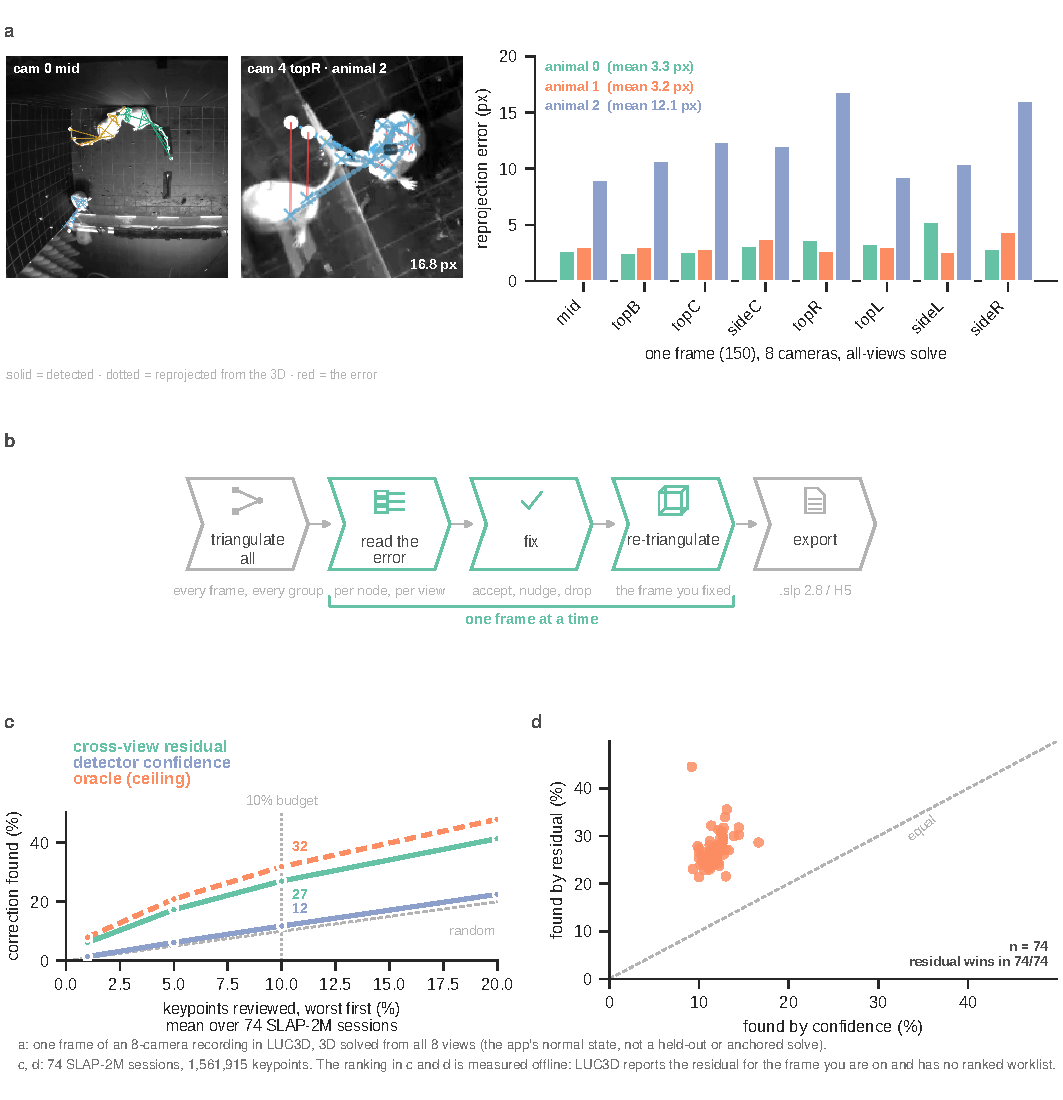
\includegraphics[width=1\textwidth]{../fig5/fig5.pdf}
  \caption{\textbf{Behavioral analysis of social rearing behavior.} Track slot 0 is male and slot 1 is female in every Mouse-Dyad-10M session; the female initiates the display in 36 of 37 sessions. \textbf{A}, One display in five views, with the 3D reconstruction. Every camera sits 58 to 76 degrees above the animals, so the height that defines the event exists only after triangulation. Only the 3D panel is metric ($230 \times 230 \times 140$~mm), and the wall of that volume nearest the viewer is drawn as edges only so the interior is seen through clear air. \textbf{B}, Time course around onset, male and female drawn separately: across-session median of per-session medians, band p25 to p75; the female reaches a higher peak nose height, 1.15 against 1.06 body lengths; the nose gap falls to 0.12 body lengths at onset. \textbf{C}, Time the female is up before the male joins, restricted to the 432 female-led displays: median 0.39~s (p25 to p75, 0.17 to 0.91~s); hatched bar, the 9\% beyond 2~s. \textbf{D}, Speed in the 0.5~s before onset, male against female, in body lengths per second: medians 0.38 and 0.23 (paired Wilcoxon $P = 6.5 \times 10^{-22}$). \textbf{E}, Facing-pursuit in the 1.5~s before onset: each animal's own body-axis orientation onto the line to its partner, scaled by that animal's own speed; negative is oriented at the partner while moving. Medians $-0.71$ (male) and $-0.06$ (female), paired Wilcoxon $P = 3.3 \times 10^{-73}$. \textbf{F}, Share of displays started, female share against male share, over the 23 sessions with six or more displays: medians 0.86 and 0.14, paired Wilcoxon $P = 2.7 \times 10^{-5}$. Pooled over all 539 displays in 37 sessions the female starts 432 of them, 80.1\%. \textbf{G}, Probability the OTHER animal is rearing at each lag, split by whose onset anchors the window, over that animal's own base rate; lines, across-session medians, band p25 to p75; far and circular-shift null curves in each panel for reference. Left, aligned to the female's onset: the male's own rearing probability, 0.6 at onset rising to 1.7 at $+0.8$~s. Right, aligned to the male's onset: the female's own rearing probability, 4.7 at onset peaking at 5.3 at $+0.3$~s. Mouse-Dyad-10M: 539 displays in 37 of 56 sessions (2 mice, 5 cameras, 150~fps); G uses 9,354 rear onsets over all 56 sessions. A display is both animals reared, neck above 0.75 body length, tail bases within 2 body lengths, held at least 0.25~s.}
  \label{fig5-standalone}
\end{figure}


\begin{thebibliography}{9}
\bibitem{Beach1976} Beach, F. A. (1976). Sexual attractivity, proceptivity, and receptivity in female mammals. \textit{Hormones and Behavior}, 7(1), 105--138.
\bibitem{Erskine1989} Erskine, M. S. (1989). Solicitation behavior in the estrous female rat: a review. \textit{Hormones and Behavior}, 23(4), 473--502.
\bibitem{McClintock1978} McClintock, M. K., \& Adler, N. T. (1978). The role of the female during copulation in wild and domestic Norway rats (\textit{Rattus norvegicus}). \textit{Behaviour}, 67(1--2), 67--96.
\end{thebibliography}

\end{document}
